\documentclass[conference]{IEEEtran} % default

\usepackage{cite} % default

\usepackage{amsmath,amssymb,amsfonts} % default

\usepackage{cleveref}
% The following formats are used so that when I call \cref{label_1} or \cref{label_1,label_2} or \crefrange{label_1}{label_4}: 
    % 1. I never get eq. or eqs. before my bracketed numbers.
    % 2. The numbers are bracketed.

% For single equation references
\crefformat{equation}{(#2#1#3)}
\Crefformat{equation}{(#2#1#3)}
% For multiple equation references
\crefmultiformat{equation}
{(#2#1#3)} % First reference
{ and (#2#1#3)} % Middle references
{ and (#2#1#3)} % Last reference
{ and (#2#1#3)} % Last reference
% For a range of equation references (e.g., (1)-(3))
\crefrangeformat{equation}{(#3#1#4) to (#5#2#6)}

\usepackage{algorithmic} % default
\usepackage{graphicx} % default

\usepackage[subpreambles=true]{standalone}
\usepackage{import}
% \usepackage{lipsum} 
\usepackage{textcomp} % default
\usepackage{xcolor} % default

\title{A Spatially Distributed Multi-Period Optimal Power Flow Analysis of Radial Active Distribution Networks with Distributed Battery Units}

% Redefine the IEEEauthorrefmark command for using numbers as superscripts
\makeatletter
\newcommand{\mysup}[1]{\@fnsymbol{#1}}
\makeatother

\author{
    \IEEEauthorblockN{
        Aryan Ritwajeet Jha\mysup{1}, \textit{Student Member, IEEE},
        Subho Paul\mysup{2}, \textit{Member, IEEE},
        Anamika Dubey\mysup{1}, \textit{Senior Member, IEEE}
        }
\IEEEauthorblockA{\IEEEauthorrefmark{1}\textit{School of Electrical Engineering \& Computer Science},
\textit{Washington State University},
Pullman, WA\\
\IEEEauthorrefmark{2}\textit{Department of Electrical Engineering},
\textit{Indian Institute of Technology (BHU) Varanasi},
Varanasi, India\\
\IEEEauthorrefmark{1}\{aryan.jha, anamika.dubey\}@wsu.edu, 
\IEEEauthorrefmark{2}\{subho.eee\}@itbhu.ac.in}
}

\begin{document}

\maketitle

% \begin{abstract}

% \textcolor{red}{insert abstract here}

% \end{abstract}

\begin{IEEEkeywords}
Batteries, distributed energy resources (DERs), distribution network, equivalent network approximation (ENApp), OpenDSS validation
\end{IEEEkeywords}

\section*{Abstract}
There has been an increasing level of interest in developing innovative and scalable algorithms for solving the Multi-Period Optimal Power Flow (MPOPF) problem in Active Distribution Systems (ADS) which can have a high penetration of Grid Edge Devices (GED) such as Solar Photovoltaics (PVs) and Battery Energy Storage Systems (BESSs). The MPOPF problem can be stated as minimizing some cost of business operation for a given time horizon subject to several constraint. In general, MPOPF problems fall into the NP-Hard class \cite{Lehmann2015Mar} due to the inherent non-linearity of powerflow physics \cite{bfm01}. Additionally, BESSs bring additional complexity into the problem by bringing in Integral constraints which arise from the fact that at a given time of participation, they can only either charge or discharge, but never both simultaneously \cite{Nazir2021Sep}. The MPOPF problem thus becomes a Mixed Integer Non Linear Programming (MINLP) problem. \\


% For a single period Optimal Power Flow (OPF) problem is concerned, many authors have proposed various kinds of relaxations to some of the constraints.

% such as solving for a linear approximation or second order conic approximation of the powerflow \cite{Baran1989Apr, Gan, Farivar, Nazir2018Jun}, relaxing the integral constraint of BESSs via a soft constraint in the objective function \cite{Nazir2018Jun, ddp_sugar_01}, etc. 

Some authors have noted that for radial distribution systems, the single period Optimal Power Flow (OPF) problem can be `spatially-decomposed' such that in order to achieve the solution to the full problem, one only needs to solve for several smaller sub-problems with periodic exchange of certain boundary variables, thereby easing computational needs, among other features \cite{Sadnan}. MPOPF problems, which are bigger than an OPF problem by a factor of the number of time-periods in the horizon, require additional techniques which can decompose the problem in order to achieve a scalable solution. \\
% Some techniques which have been previously proposed include modelling the MPOPF problem as a Multi Period Control problem and solving it using Differential Dynamic Programming \cite{ddp_sugar_01}. Other authors have proposed solving for the entire horizon via scalable linearized algorithms and using the resulting values of temporally-coupled variables as set-points for a more involved, but temporally-decoupled OPF analysis for each time-step \cite{Nazir2018Jun, Nazir2019Jun}.

In this poster, we present Multi-Period ENApp, based on the ENApp algorithm proposed in \cite{Sadnan} for the MPOPF problem for BESS-equipped ADSs. Preliminary results of this `Mulit-Period ENApp' algorithm, which have been validated against both a brute-forced benchmark optimization model for optimality gap, as well as against OpenDSS for feasibility and modelling consistency, have been promising, with faster solution times but without compromising on optimality or feasiblity of the problem. 

\section*{Key Figures}

\begin{figure}[h]
    \centering
    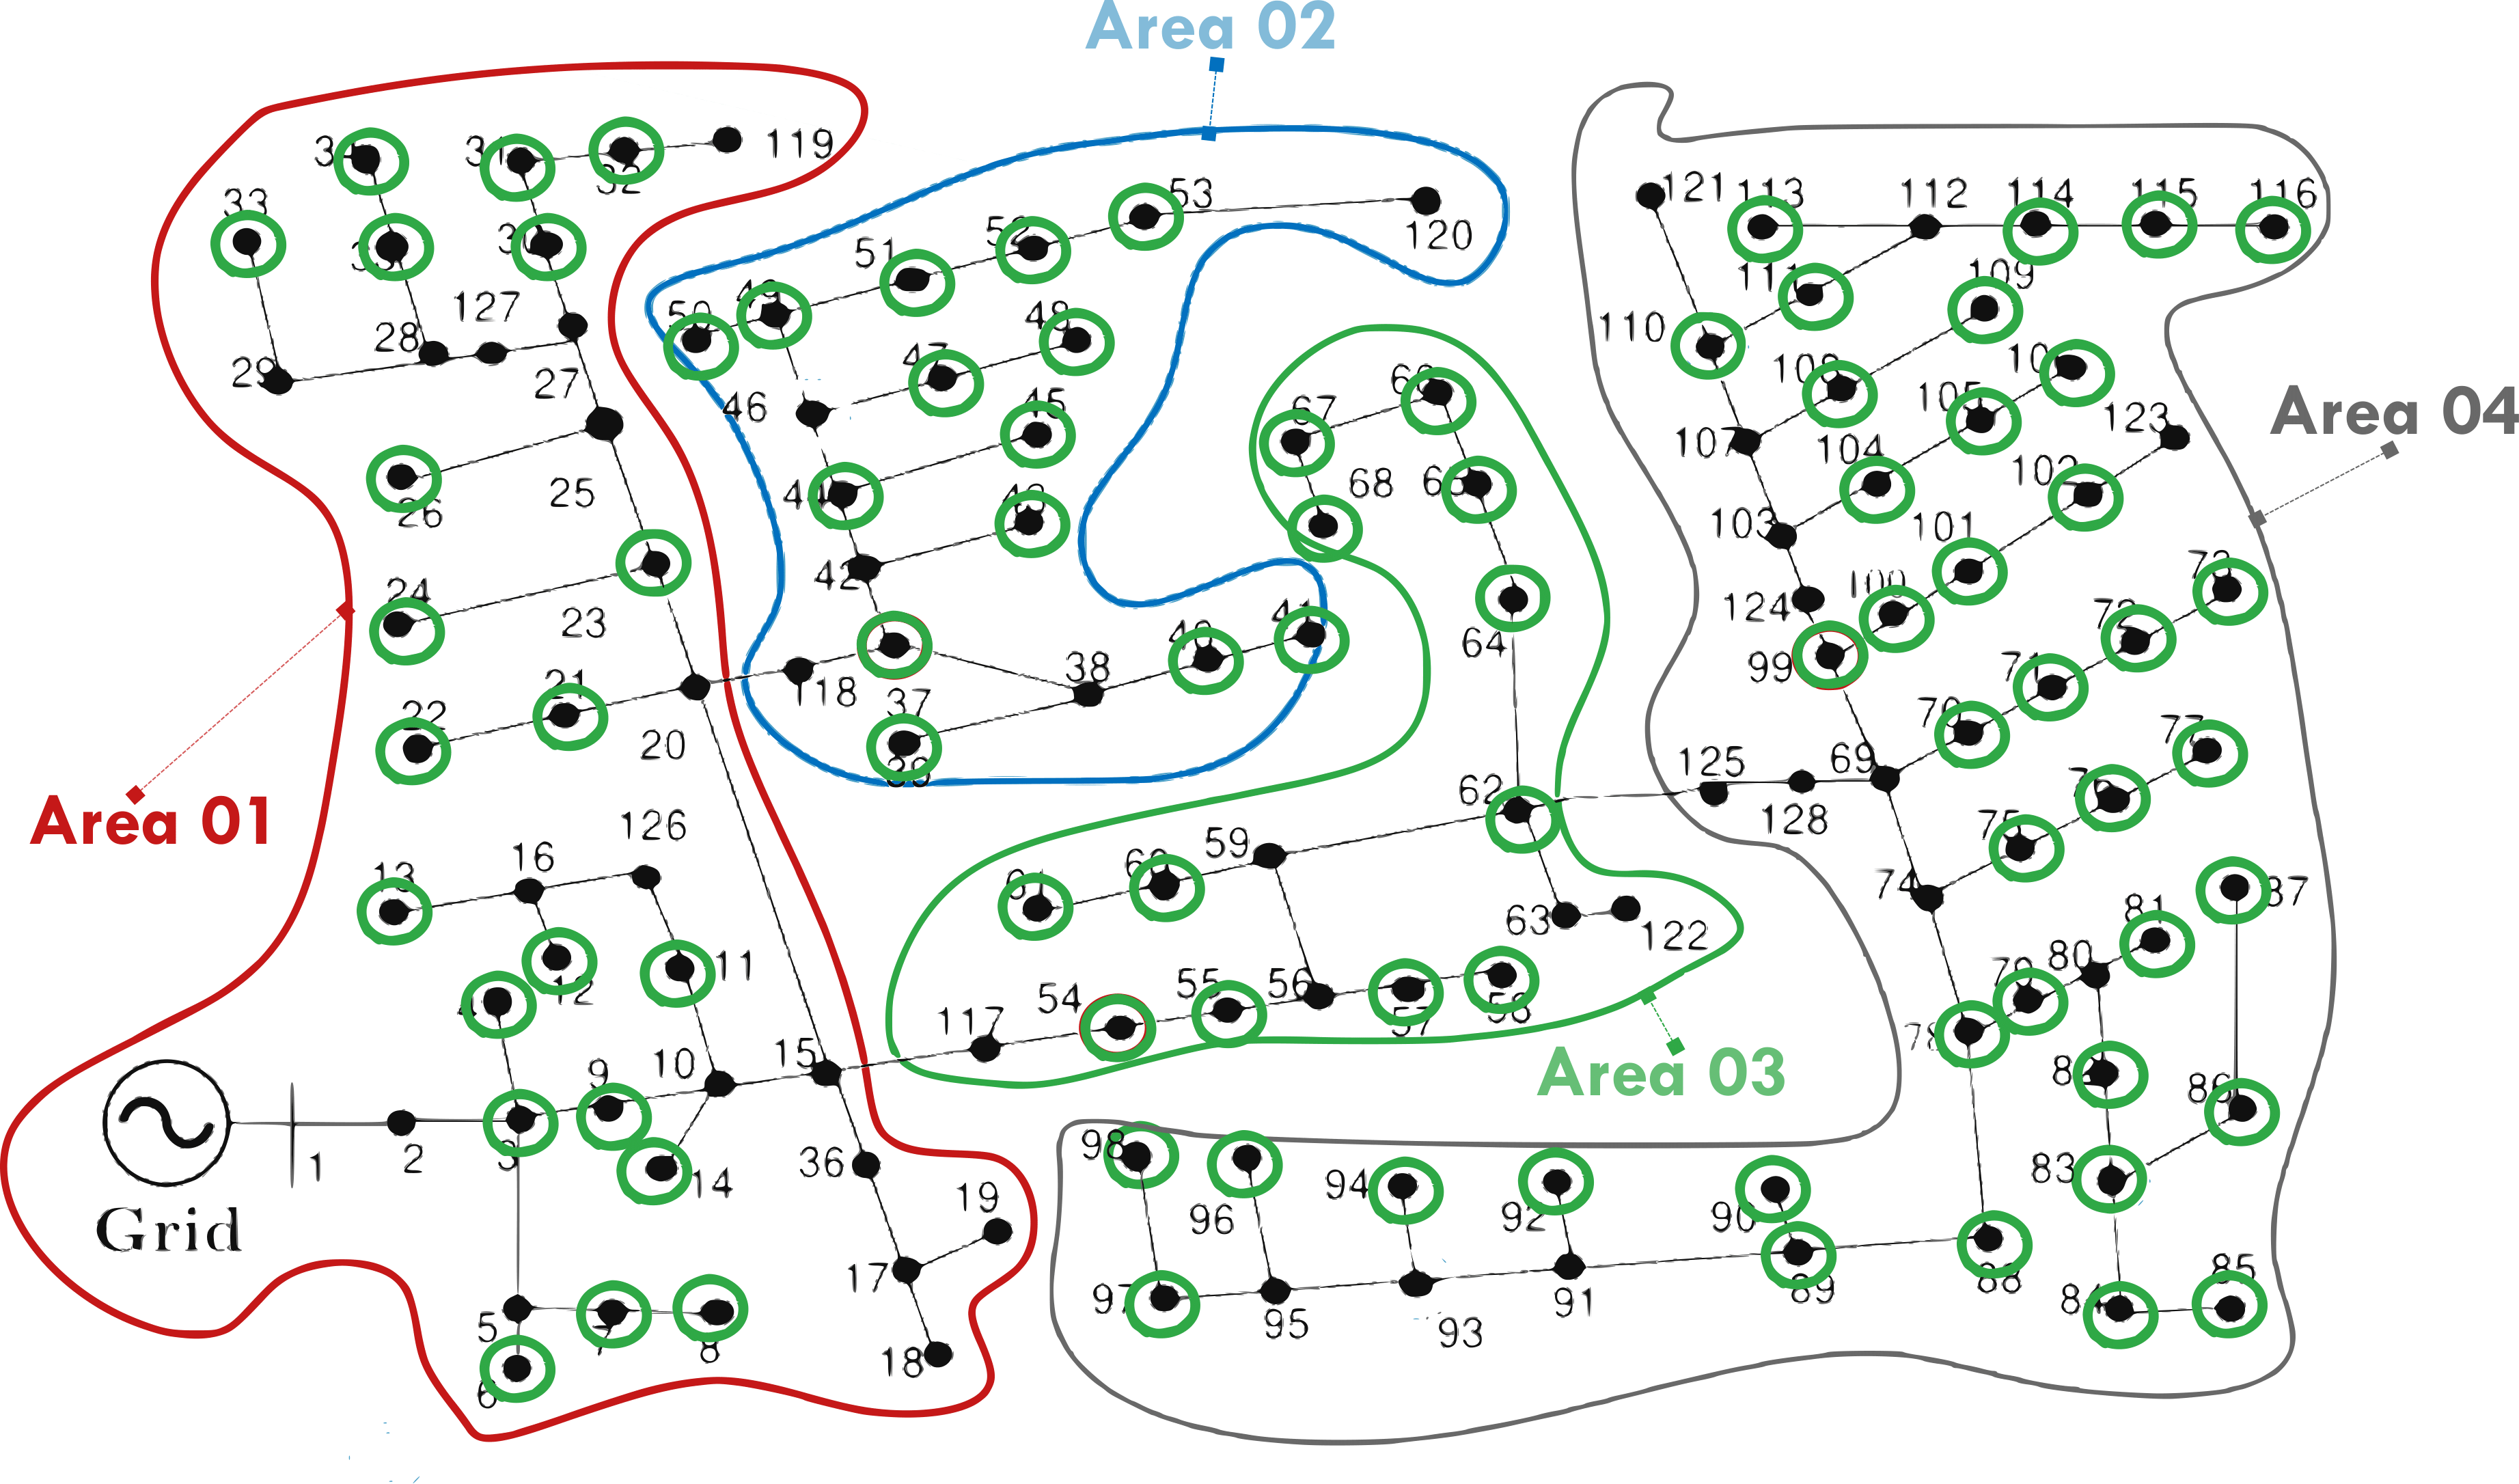
\includegraphics[width=0.4\textwidth]{figures/ieee123-FourAreas.png}
    \caption{Division of the IEEE 123 Node System into Four Areas}
    \label{fig:ieee123-four-areas}
\end{figure}

\begin{figure}[h]
    \centering
    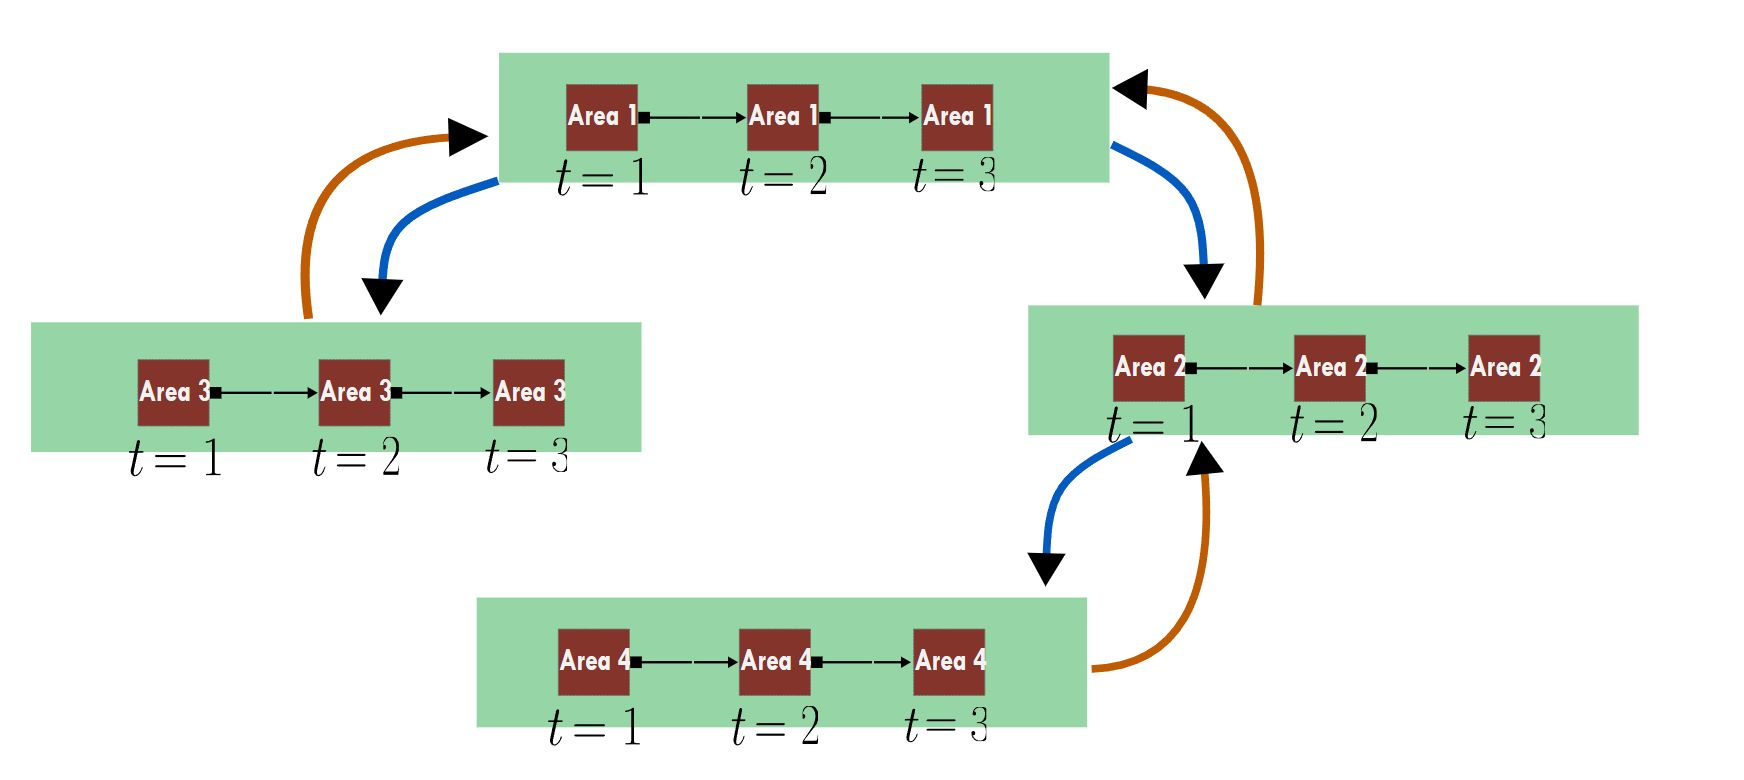
\includegraphics[width=0.4\textwidth]{figures/mpopf-spatially-distributed-temporally-brute-forced.jpg}
    \caption{Schematic describing the workflow of the Multi Period ENApp algorithm for a 3-time-step horizon for the system as divided as per \Cref{fig:ieee123-four-areas}.}
    \label{fig:mpenapp}
\end{figure}

\bibliographystyle{IEEEtran}
\bibliography{bibFile}

\end{document}
